 %!TEX program = xelatex
 % 使用 ctexart 文类,UTF-8 
 % 作者:王泽宇
\documentclass[UTF8]{ctexart}
\usepackage{tikz,mathpazo}
\usetikzlibrary{shapes.geometric, arrows}
\usepackage{flowchart}
\begin{document}
\begin{tikzpicture}[font={\sf \small}]
\def \smbwd{2cm}
\thispagestyle{empty}

 %定义流程图的具体形状
\node (start) at (0,0) [draw, terminal,minimum width=\smbwd, minimum height=0.5cm] {开始};      % 定义开始 
\node (getdata) at (0,-1.5) [draw, predproc, align=left,minimum width=\smbwd,minimum height=1cm] {读取数据};        %定义预处理过程,读取数据
\node (decide) at (0,-3.5) [draw, decision, minimum width=\smbwd, minimum height=1cm] {判断条件};    %定义判断条件
\node (storage) at (0,-5.5) [draw, storage, minimum width=\smbwd, minimum height=1cm] {数据存储};     %定义数据存储
\node (process) at (3,-5.5) [draw, process, minimum width=\smbwd, minimum height=1cm] {处理过程};      %定义处理过程
\coordinate (point1) at (0,-6.75);
\node (end) at (0,-7.75) [draw, terminal,minimum width=\smbwd,minimum height=0.5cm] {结束};        %定义结束

 %连接定义的形状,绘制流程图--表示垂直线,|表示箭头方向
\draw[->] (start) -- (getdata);
\draw[->] (getdata) -- (decide);
\draw[->] (decide) -| node[above]{是} (process);
\draw[->] (decide) -- node[left]{否}(storage);
\draw[->] (process) |- (point1);
\draw[->] (storage) -- (point1) -- (end);
\end{tikzpicture}

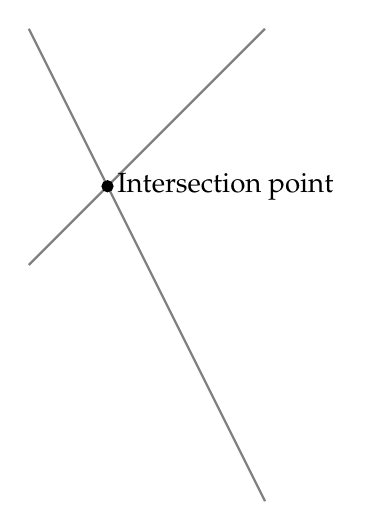
\begin{tikzpicture}
\draw[gray, thick] (-1,2) -- (2,-4);
\draw[gray, thick] (-1,-1) -- (2,2);
\filldraw[black] (0,0) circle (2pt) node[anchor=west] {Intersection point};

\end{tikzpicture}

\end{document}